\section{Desarrollo } 

\begin{itemize}
\item Tarea 1 : Conectar a SQL Server desde Power BI Desktop


\begin{enumerate}
\item Inciar Power BI Desktop

\begin{center}
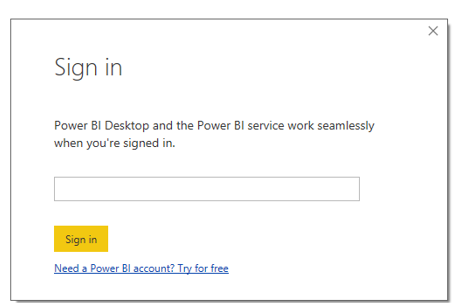
\includegraphics[scale=0.55]{./Imagenes/a1.png}
\end{center}

\item Cuando la Ventana de Power BI Desktop aparezca, en el panel a mano izquierda, hacer click en ObtenerDatos (Get Data).

\begin{center}
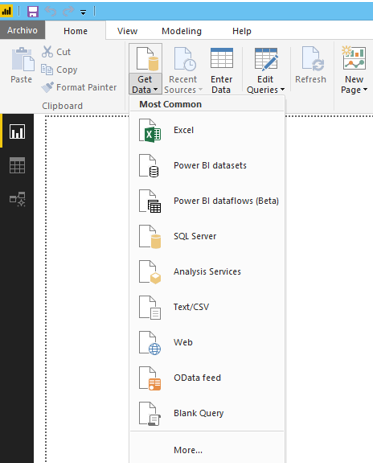
\includegraphics[scale=0.55]{./Imagenes/a2.png}
\end{center}


\item En el cuadro de dialogo Obtener Datos (Get Data), click en base de datos SQL Server, y luego hacer click en Conectar (Connect).

\begin{center}
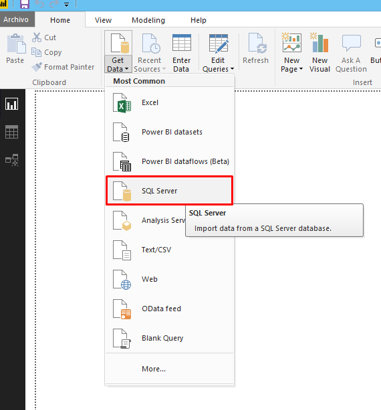
\includegraphics[scale=0.55]{./Imagenes/a3.png}
\end{center}


\item En el cuadro de dialogo base de datos SQL Server, en la casilla servidor tipear (local), en la casilla Base de datos (opcional) / Database (optional), tipear AdventureWorks2017, y hacer clic en OK.

\begin{center}
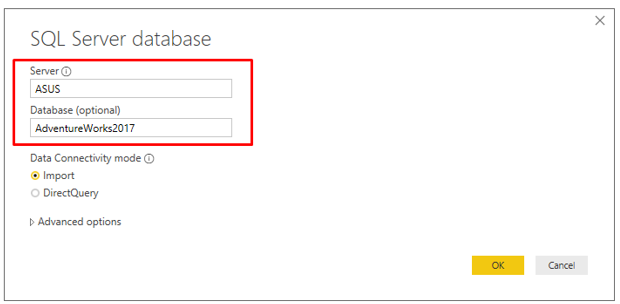
\includegraphics[scale=0.55]{./Imagenes/a4.png}
\end{center}

\item En el cuadro de dialogo base de datos SQL Server, aceptar los valores por defecto, y luego click en el Conectar (Connect). Si un mensaje de Soporte de Encriptación es visualizado, hacer click en OK.

\begin{center}
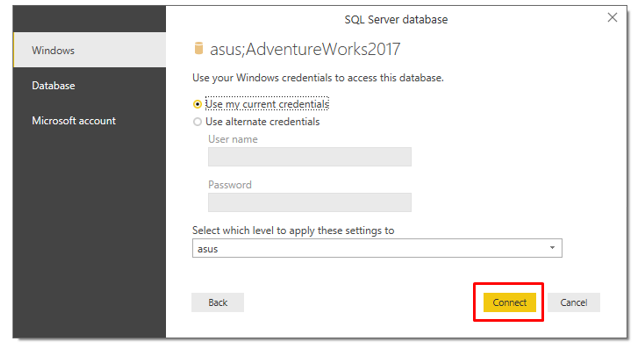
\includegraphics[scale=0.55]{./Imagenes/a5.png}
\end{center}
\begin{center}
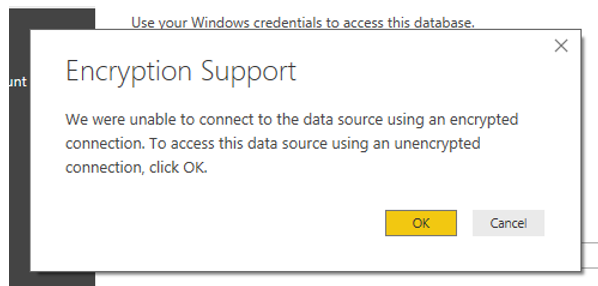
\includegraphics[scale=0.55]{./Imagenes/5aa.png}
\end{center}

\item En el cuadro de dialogo Navegador (Navigator), seleccionar el check en Sales.vSalesPerson, y entonces hacer click en Cargar (Load).

\begin{center}
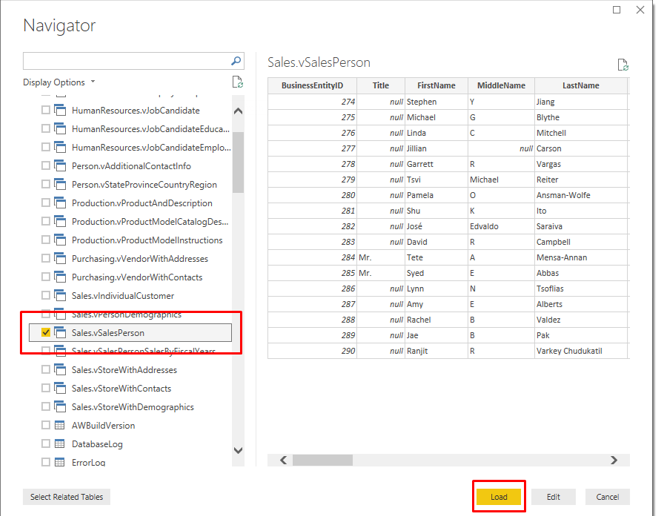
\includegraphics[scale=0.55]{./Imagenes/a6.png}
\end{center}


\item En el panel Campos (Fields), expandir Sales vSalesPerson para ver todas las columnas.

\begin{center}
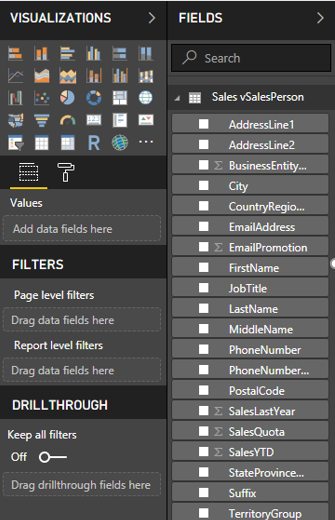
\includegraphics[scale=0.55]{./Imagenes/a7.png}
\end{center}


\item En el menu principal (Home ribbon), hacer click en Funetes Recientes (Recent Sources), y en local:AdventureWorks2017. 

\begin{center}
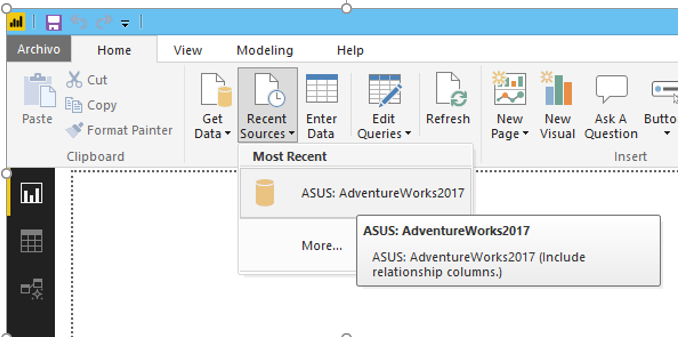
\includegraphics[scale=0.55]{./Imagenes/a8.png}
\end{center}

\item En el cuadro de dialogo Navegador (Navigator), seleccionar la vista Sales.vStoreWithDemographics, y luego hacer click en Cargar (Load).

\begin{center}
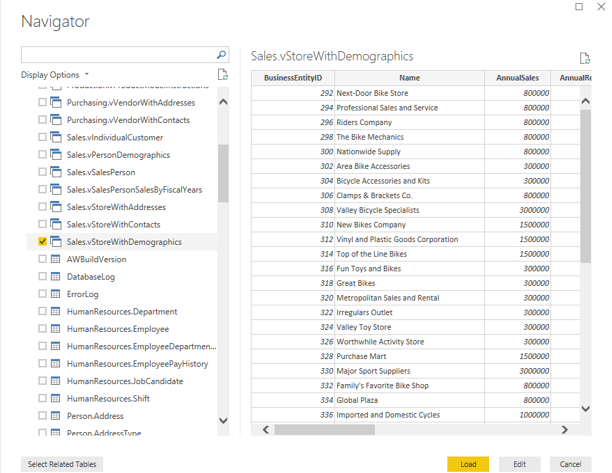
\includegraphics[scale=0.55]{./Imagenes/a9.png}
\end{center}

\item En el panel Campos (Fields), expandir Sales.vStoreWithDemographics para ver todas las columnas.
\begin{center}
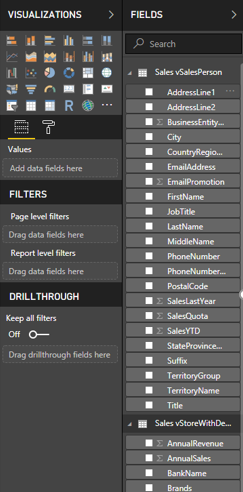
\includegraphics[scale=0.55]{./Imagenes/a10.png}
\end{center}

\item En el menu principal (Home ribbon), hacer click en Obtener Datos (Get Data), y luego click en SQL Server. 

\begin{center}
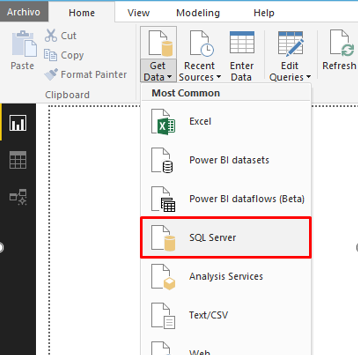
\includegraphics[scale=0.55]{./Imagenes/a11.png}
\end{center}

\item En el cuadro dialogo base de datos SQL Server, en la casilla Servidor (Server), tipear (local), y en la casilla Base de datos (opcional), tipear AdventureWorks2017.

\begin{center}
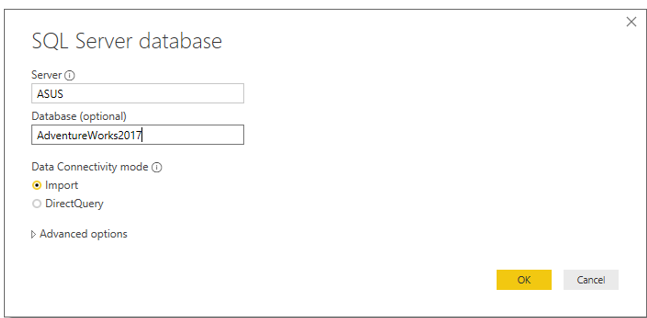
\includegraphics[scale=0.55]{./Imagenes/a12.png}
\end{center}

\item Expandir opciones Avanzadas, en la casilla sentencia SQL (opcional, base de datos requerida), tipear la
siguiente consulta, y luego hacer click en OK:
SELECT TOP 10 P.ProductID, P.Name AS Product, SUM(CAST(LineTotal AS decimal(18,2))) AS LineTotal FROM
Purchasing.PurchaseOrderDetail AS POD INNER JOIN Production.Product AS P ON POD.ProductID = P.ProductID
GROUP BY P.ProductID, P.Name ORDER BY LineTotal DESC


\begin{center}
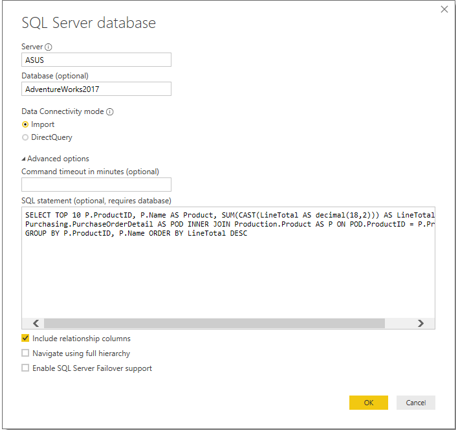
\includegraphics[scale=0.55]{./Imagenes/a13.png}
\end{center}

\item En el cuadro de dialogo (local): AdventureWorks2017 hacer click en Cargar (Load).En el cuadro de dialogo (local): AdventureWorks2017 hacer click en Cargar (Load).


\begin{center}
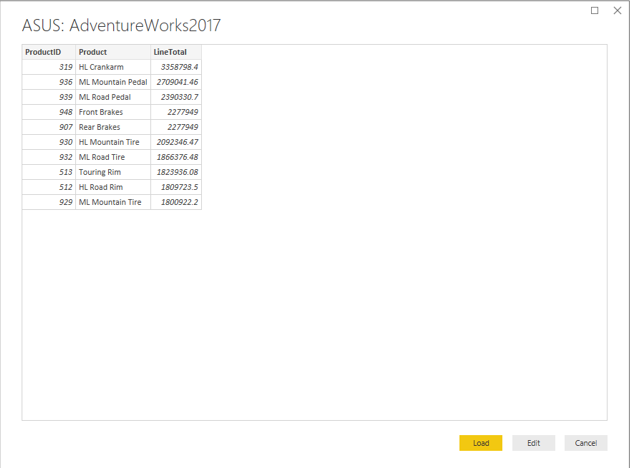
\includegraphics[scale=0.55]{./Imagenes/a14.png}
\end{center}

\item En el panel Campos, expander Query1 para ver todas las columnas.


\begin{center}
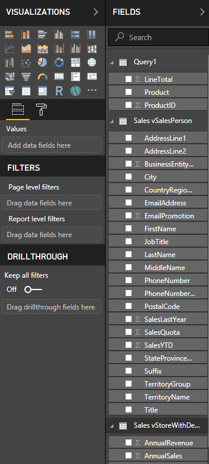
\includegraphics[scale=0.55]{./Imagenes/a15.png}
\end{center}


\item Hacer click en la elipsis (…) al lado de Query1 y hacer click en Renombrar, tipear Top 10 Productos Vendidos, y presionar Enter.


\begin{center}
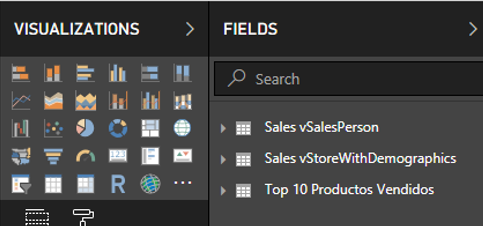
\includegraphics[scale=0.55]{./Imagenes/a16.png}
\end{center}



\end{enumerate}








\item Tarea 2 : Adicioar Graficos Al Reporte
\begin{enumerate}

\item En el panel Visualizaciones (Visualizations), hacer click en el gráfico Columna apilada (Stacked column) para añadir el control al reporte.
\begin{center}
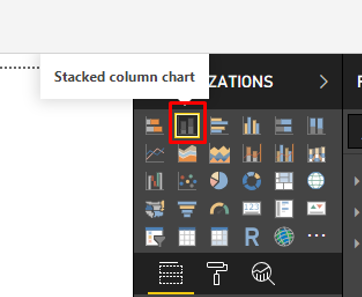
\includegraphics[scale=0.55]{./Imagenes/1.png}
\end{center}


\item En el panel Campos (Fields), bajo Sales vSalesPerson, arrastrar el campo FirstName a la casilla Eje (Axis) en el panel de Visualización (Visualizations).
\begin{center}
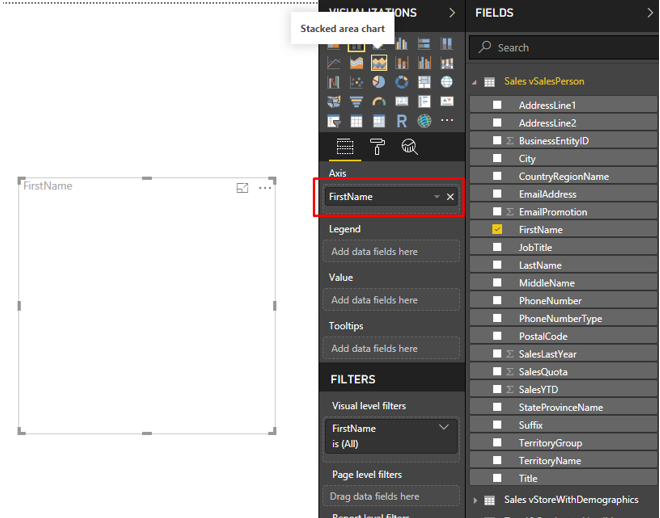
\includegraphics[scale=0.55]{./Imagenes/2.png}
\end{center}

\item Arrastrar el campo SalesYTD a la casilla Valores (Values). El gráfico se llenará con datos.
\begin{center}
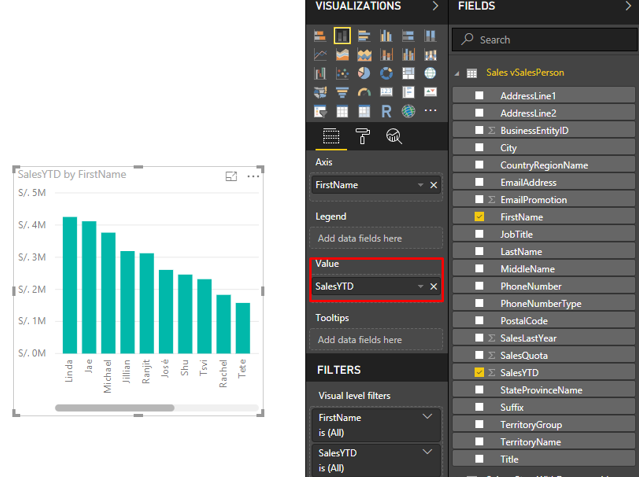
\includegraphics[scale=0.55]{./Imagenes/3.png}
\end{center}

\item En el gráfico en el reporte, ajustar el tamaño del gráfico para que muestre a todo el personal de ventas.
\begin{center}
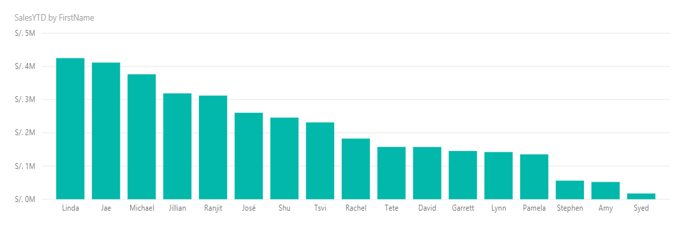
\includegraphics[scale=0.55]{./Imagenes/4.png}
\end{center}

\item Asegurarse que el gráfico tiene el foco y luego ir al panel de Visualización (Visualizations), hacer click en la pestaña Formato (Format).
\begin{center}
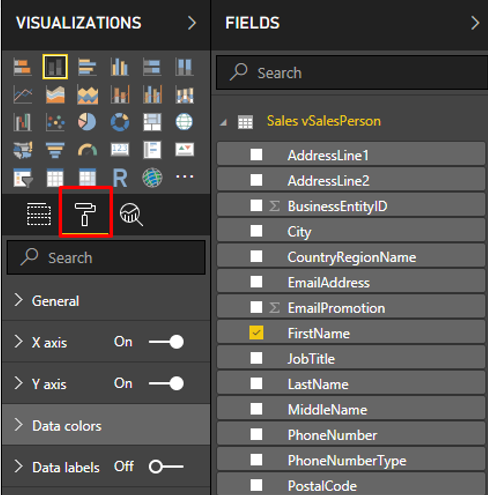
\includegraphics[scale=0.55]{./Imagenes/5.png}
\end{center}

\item Expandir Colores de datos (Data colors), activar la opción Mostrar todos (Show all).
\begin{center}
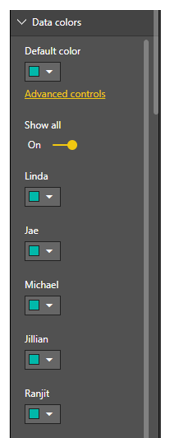
\includegraphics[scale=0.55]{./Imagenes/6.png}
\end{center}

\item Cambiar el color para Jae, Linda, y Michael a rojo.
\begin{center}
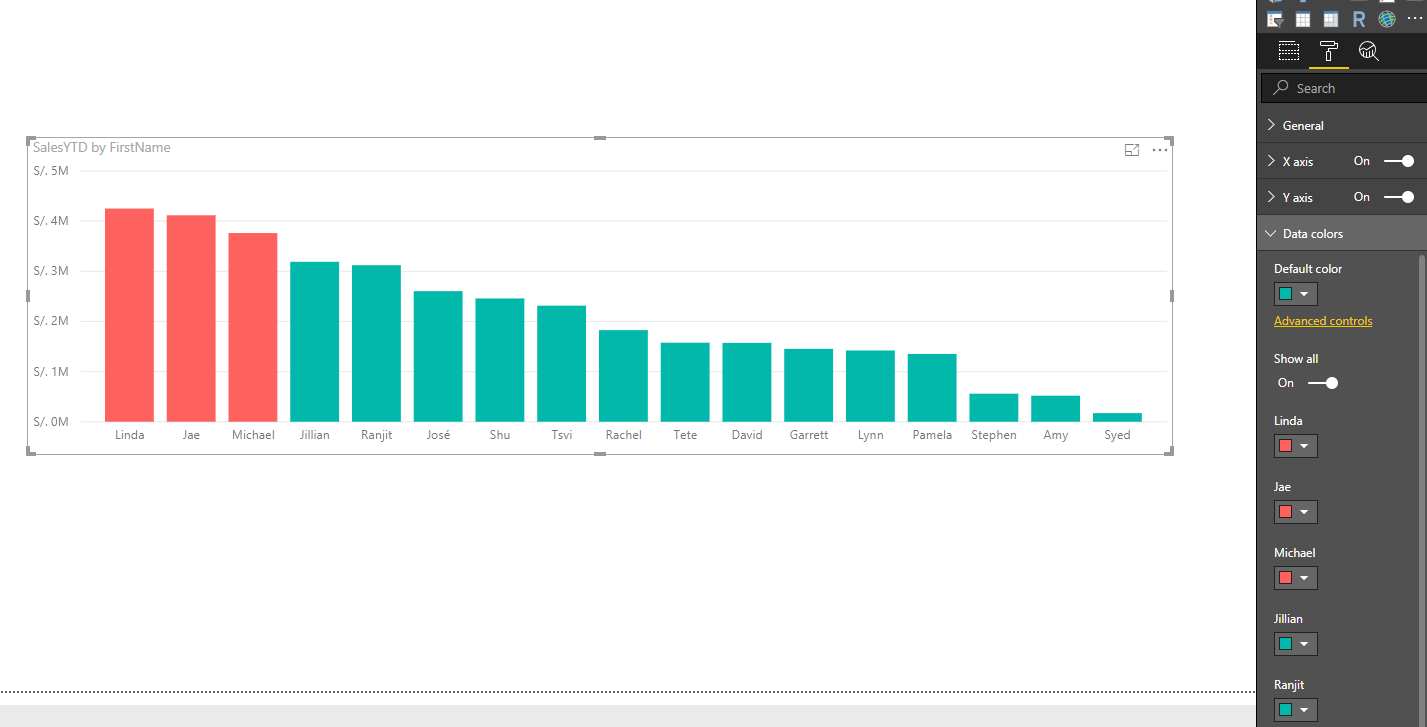
\includegraphics[scale=0.55]{./Imagenes/7.png}
\end{center}

\item Hacer click en el área de reporte y luego en el panel de Visualizaciones (Visualizations pane), hacer clic en el gráfico Pie para añadir el control al reporte. Arrastrar el gráfico Pie al lado derecho del gráfico de barras o debajo si no hubiese espacio. 
\begin{center}
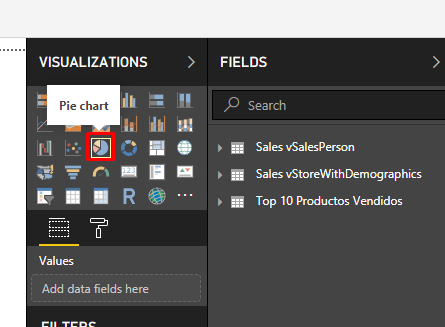
\includegraphics[scale=0.55]{./Imagenes/8.png}
\end{center}

\item  En el panel Campos (Fields pane), bajo Sales vStoreWithDemographics, arrastrar el campo Specialty a la casilla Leyenda (Legend) en el panel de Visualizaciones.
\begin{center}
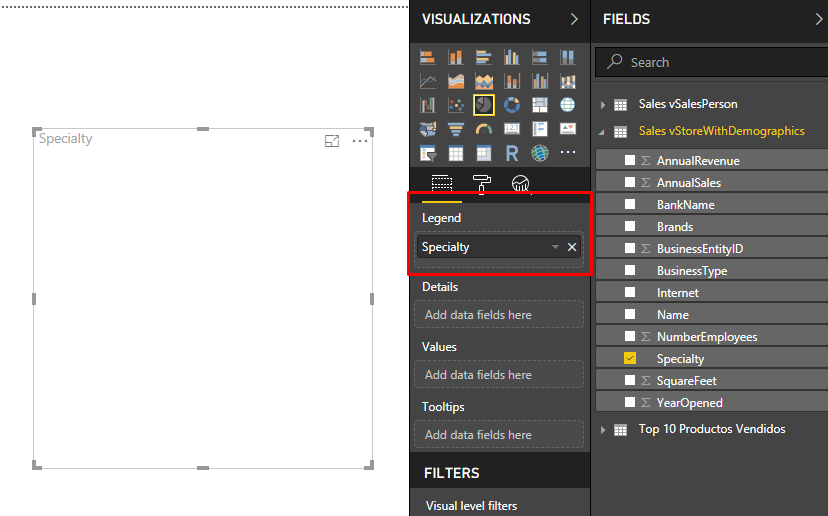
\includegraphics[scale=0.55]{./Imagenes/9.png}
\end{center}

\item Arrastrar el campo NumberEmployees a la casilla Valores (Values). El gráfico se llenará con los datos y mostrará tres secciones.
\begin{center}
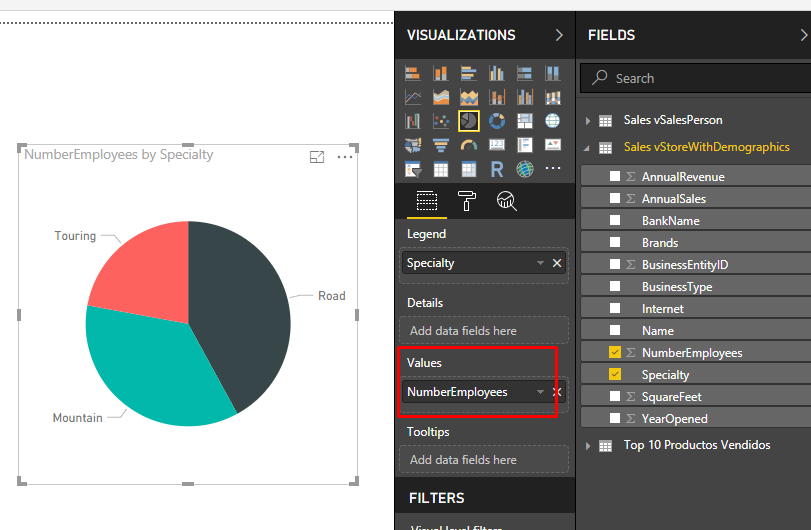
\includegraphics[scale=0.55]{./Imagenes/10.png}
\end{center}

\item Nuevamente click en el área de reporte, luego ir al panel de Visualizaciones y añadir otro gráfico de Columna apilada (Stacked columna) al reporte. Este gráico debe estar debajo de los gráficos previos.
\begin{center}
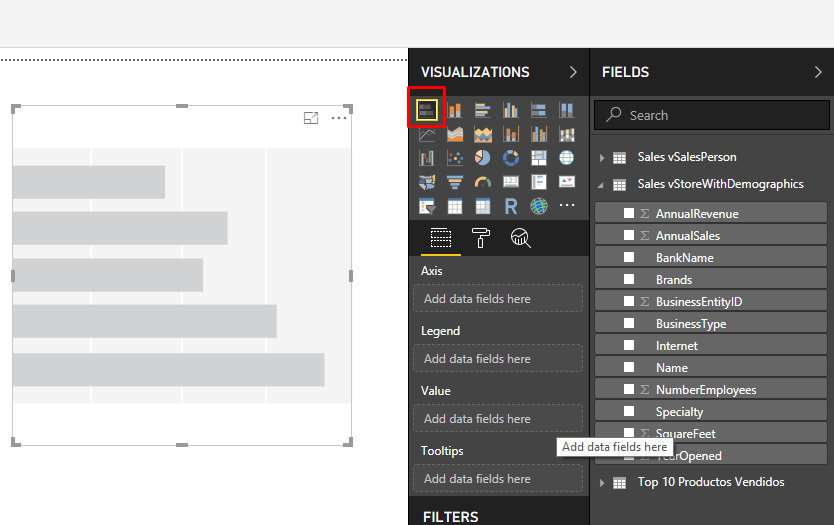
\includegraphics[scale=0.55]{./Imagenes/11.png}
\end{center}


\item En el panel Campos, expander Top 10 Productos Vendidos, arrastrar el campo Product a la casilla Eje (Axis) en el panel de Visualizaciones.
\begin{center}
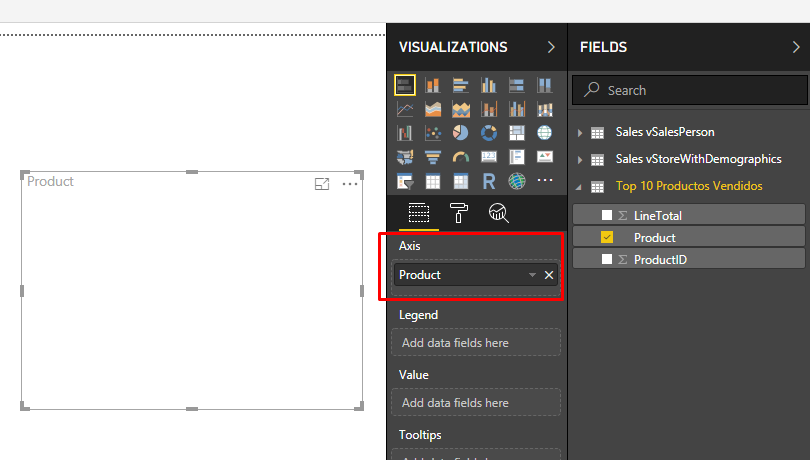
\includegraphics[scale=0.55]{./Imagenes/12.png}
\end{center}

\item Arrastrar el campo LineTotal a la casilla Valores (Value). El gráfico se llenara con datos.Arrastrar el campo LineTotal a la casilla Valores (Value). El gráfico se llenara con datos.
\begin{center}
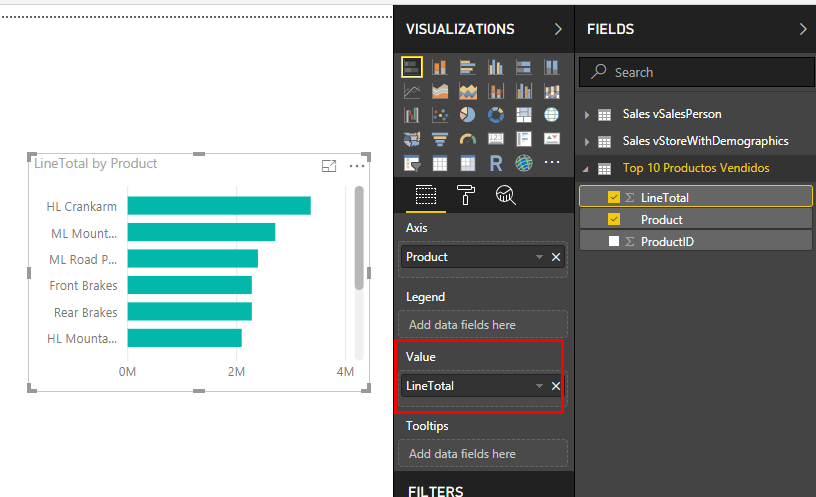
\includegraphics[scale=0.55]{./Imagenes/13.png}
\end{center}

\item Hacer click en el gráfico Top 10 Productos vendidos, entonces en el Panel de Visualizaciones, hacer click en el gráfico Donut. Revisar que fácil alternar un tipo de gráfico diferente
\begin{center}
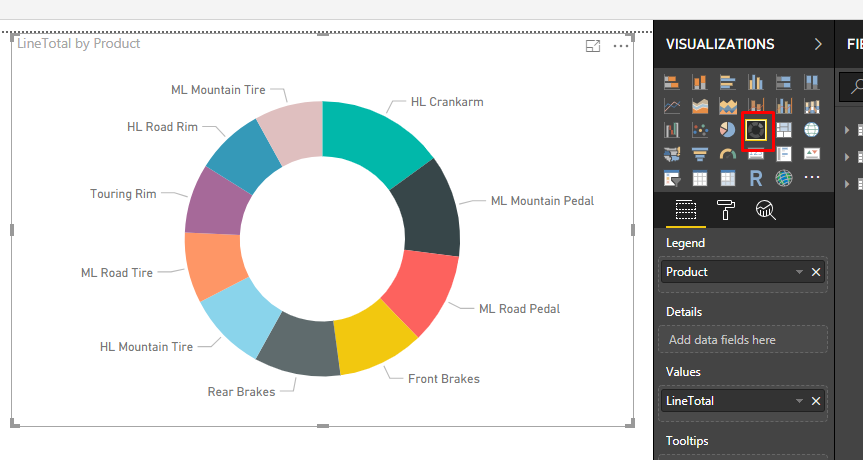
\includegraphics[scale=0.55]{./Imagenes/14.png}
\end{center}

\item En el gráfico, ajustar el tamaño para que se puedan visualizer todos los nombres de productos en el gráfico de Donut.
\begin{center}
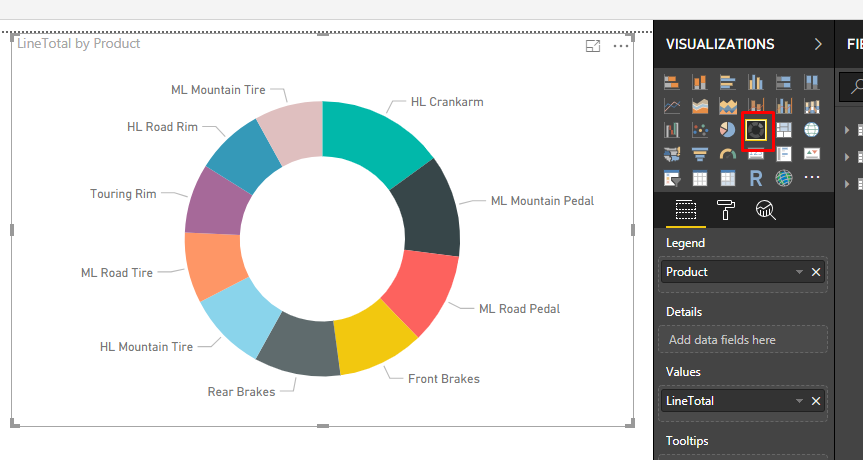
\includegraphics[scale=0.55]{./Imagenes/14.png}
\end{center}

\item En el panel Campos, bajo Sales vStoreWithDemographics, hacer click y arrastrar el campo AnnualSales directamente al área de reportes. Verificar como se crea automaticamente un gráfico de barras.
\begin{center}
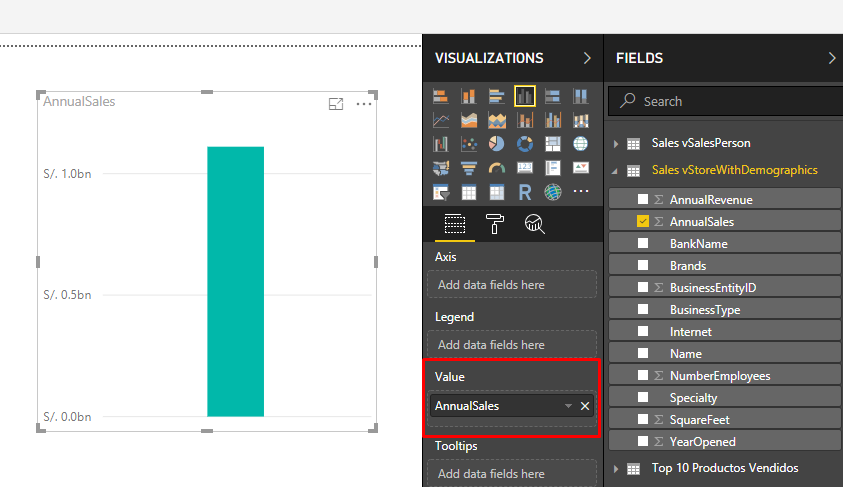
\includegraphics[scale=0.55]{./Imagenes/16.png}
\end{center}

\item En el panel Campos, seleccionar la casilla de verificación de AnnualRevenue, y apreciar que este adiciona el campo al gráfico de barras.
\begin{center}
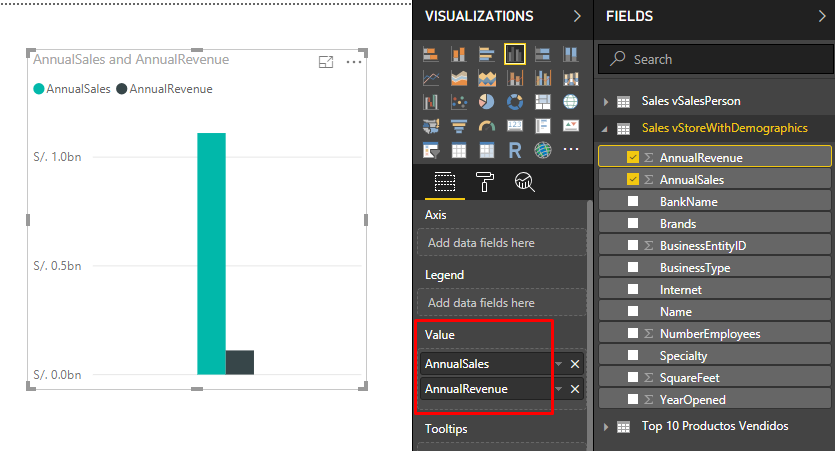
\includegraphics[scale=0.55]{./Imagenes/17.png}
\end{center}

\item En el panel Campos, hacer click en la elipsis (…) contigua a AnnualRevenue, y hacer click en Renombrar (Rename). Tipear Beneficios anuales luego presionar Enter.
\begin{center}
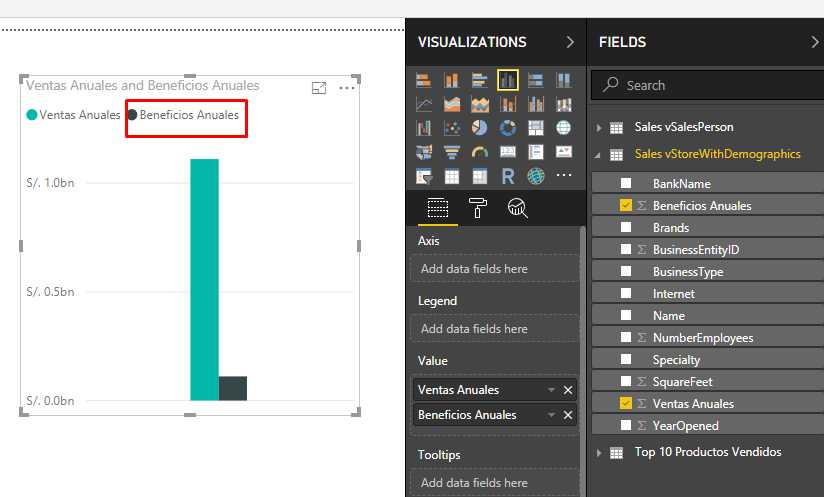
\includegraphics[scale=0.55]{./Imagenes/18.png}
\end{center}

\item Repetir el paso 18, para renombrar el campo AnnualSales a Ventas Anuales. Apreciar que los nombres en los titulus y leyenda del gráfico de barras se han actualizado.
\begin{center}
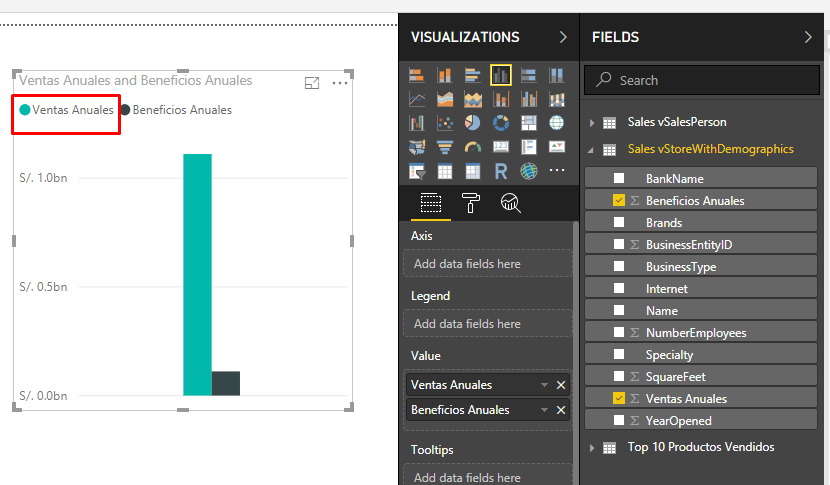
\includegraphics[scale=0.55]{./Imagenes/19.png}
\end{center}

\item Hacer click en el área de reporte, luego en el panel de Visualizaciones y en la pestaña Formato (Format).
\begin{center}
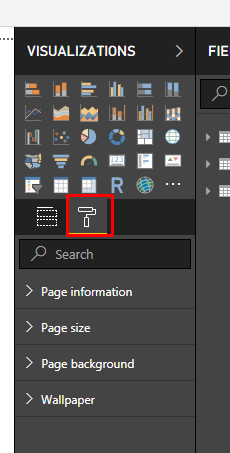
\includegraphics[scale=0.55]{./Imagenes/20.png}
\end{center}

\item Expandir la Información de página (Page Information), y en la casilla Nombre tipear Ventas. Hacer click en el área de reporte y apreciar que el nombre ha cambiado en la pestaña al final del reporte.
\begin{center}
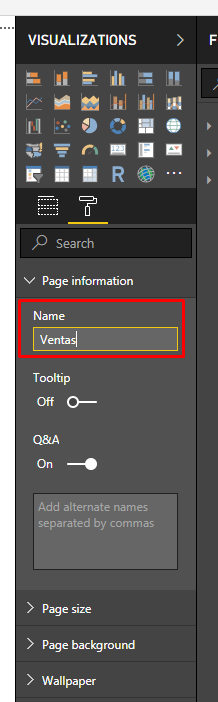
\includegraphics[scale=0.55]{./Imagenes/21.png}
\end{center}

\item En el menu Archivo (File menu), hacer click en Guardar (Save), crear un directorio Power BI, y guardar el archive como Ventas de Adventure Works Sales.
\begin{center}
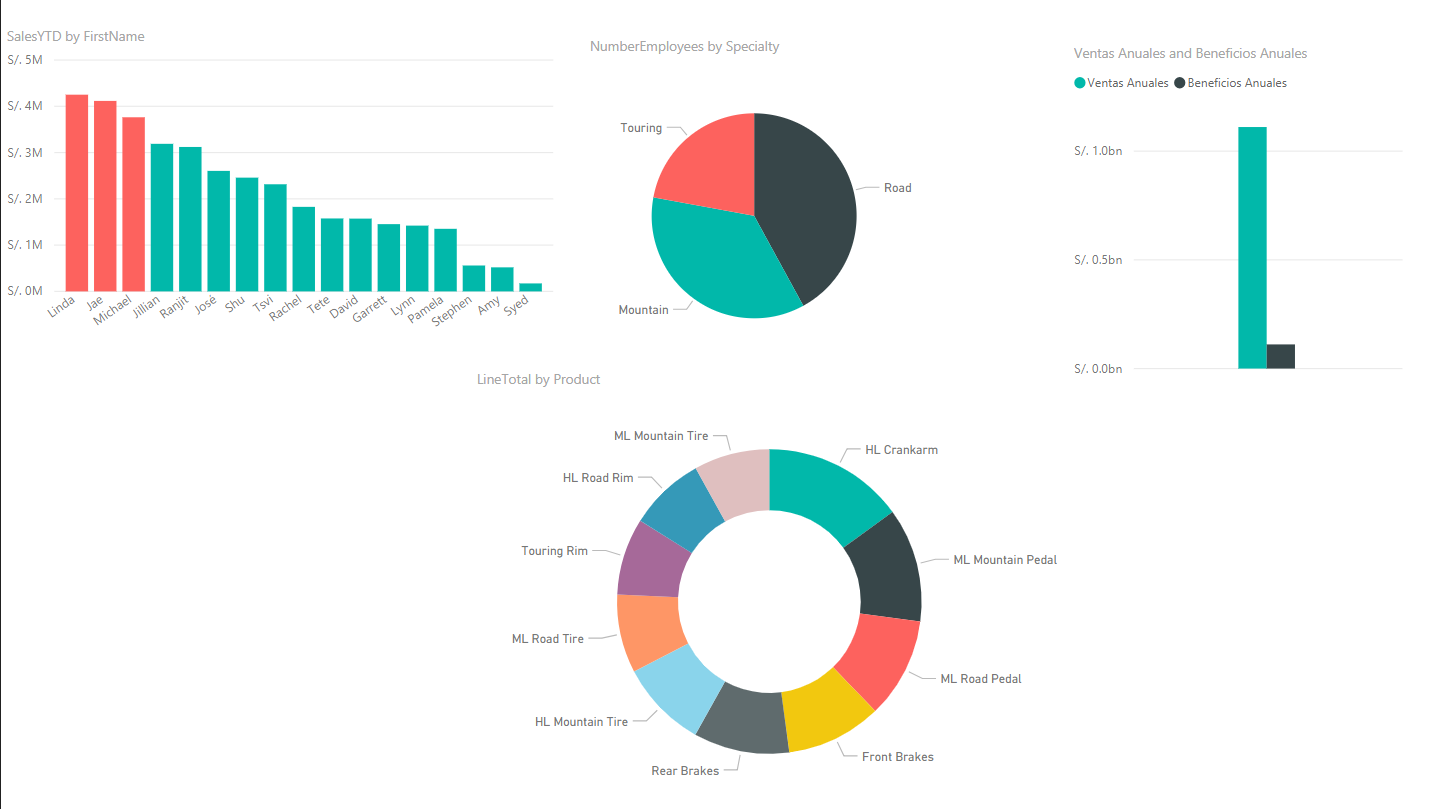
\includegraphics[scale=0.55]{./Imagenes/21a.png}
\end{center}
\begin{center}
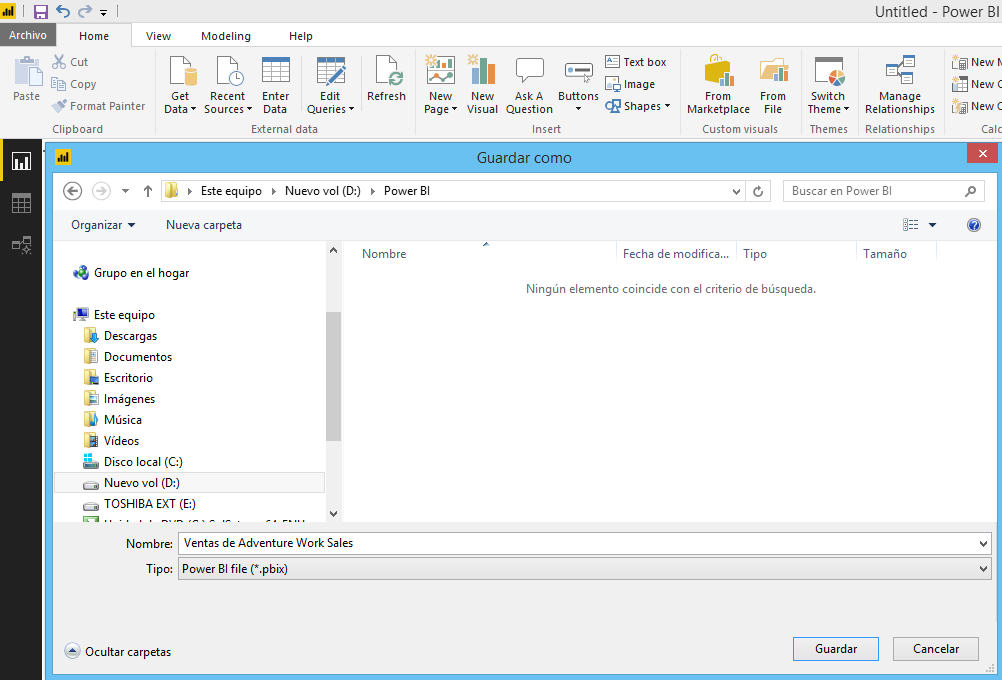
\includegraphics[scale=0.55]{./Imagenes/22.png}
\end{center}





\end{enumerate}




\item Tarea 3 : Publicar el reporte en el PowerBI
\begin{enumerate}

\item En el menu principal (Home ribbon), hacer click en Publica (Publish).
\begin{center}
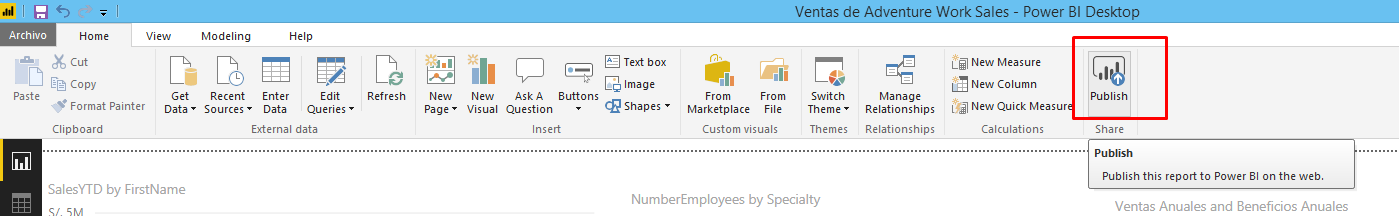
\includegraphics[scale=0.30]{./Imagenes/23.png}
\end{center}

\item Si pregunta por Guardar los cambios, hacer click en Guardar (Save).
\begin{center}
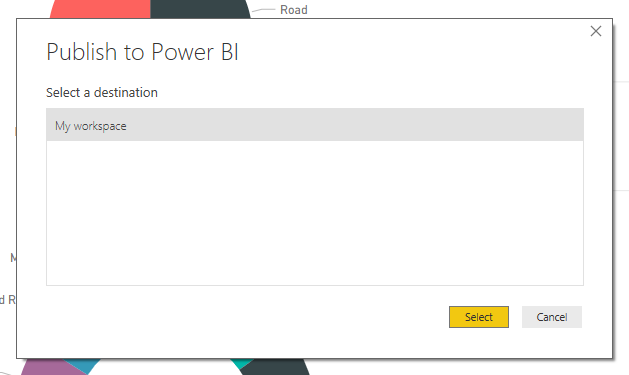
\includegraphics[scale=0.55]{./Imagenes/24.png}
\end{center}

\item El reporte será publicado en el Portal de Power BI. Cuando la ventana muestre Satisfactorio (9Success), hacer click en Abrir (Open) 'Ventas Adventure Works.pibx' en Power BI para ver el reporte en línea.
\begin{center}
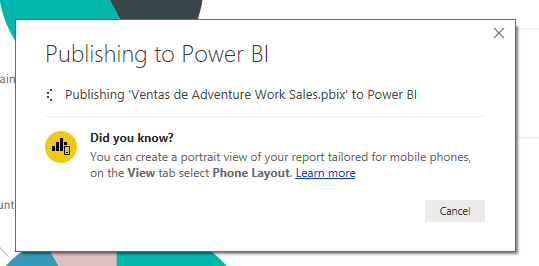
\includegraphics[scale=0.55]{./Imagenes/25.png}
\end{center}
\begin{center}
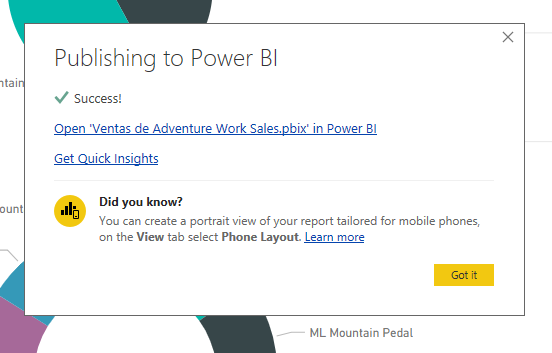
\includegraphics[scale=0.55]{./Imagenes/26.png}
\end{center}

\item Cuando el navegador se abra, hacer click en Iniciar Sesión, ingresar su correo y contraseña, Iniciar sesión, y esperar a que el reporte abra en Internet Explorer
\begin{center}
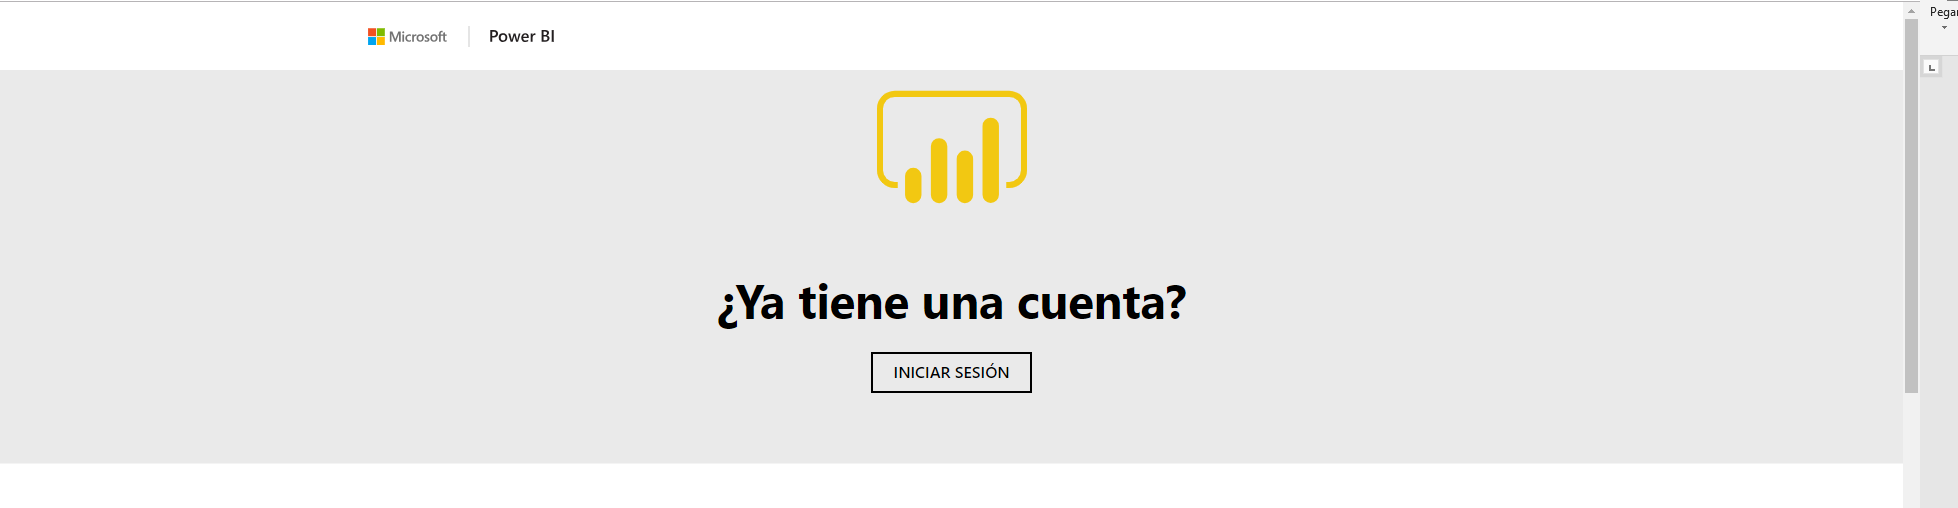
\includegraphics[scale=0.30]{./Imagenes/27.png}
\end{center}
\begin{center}
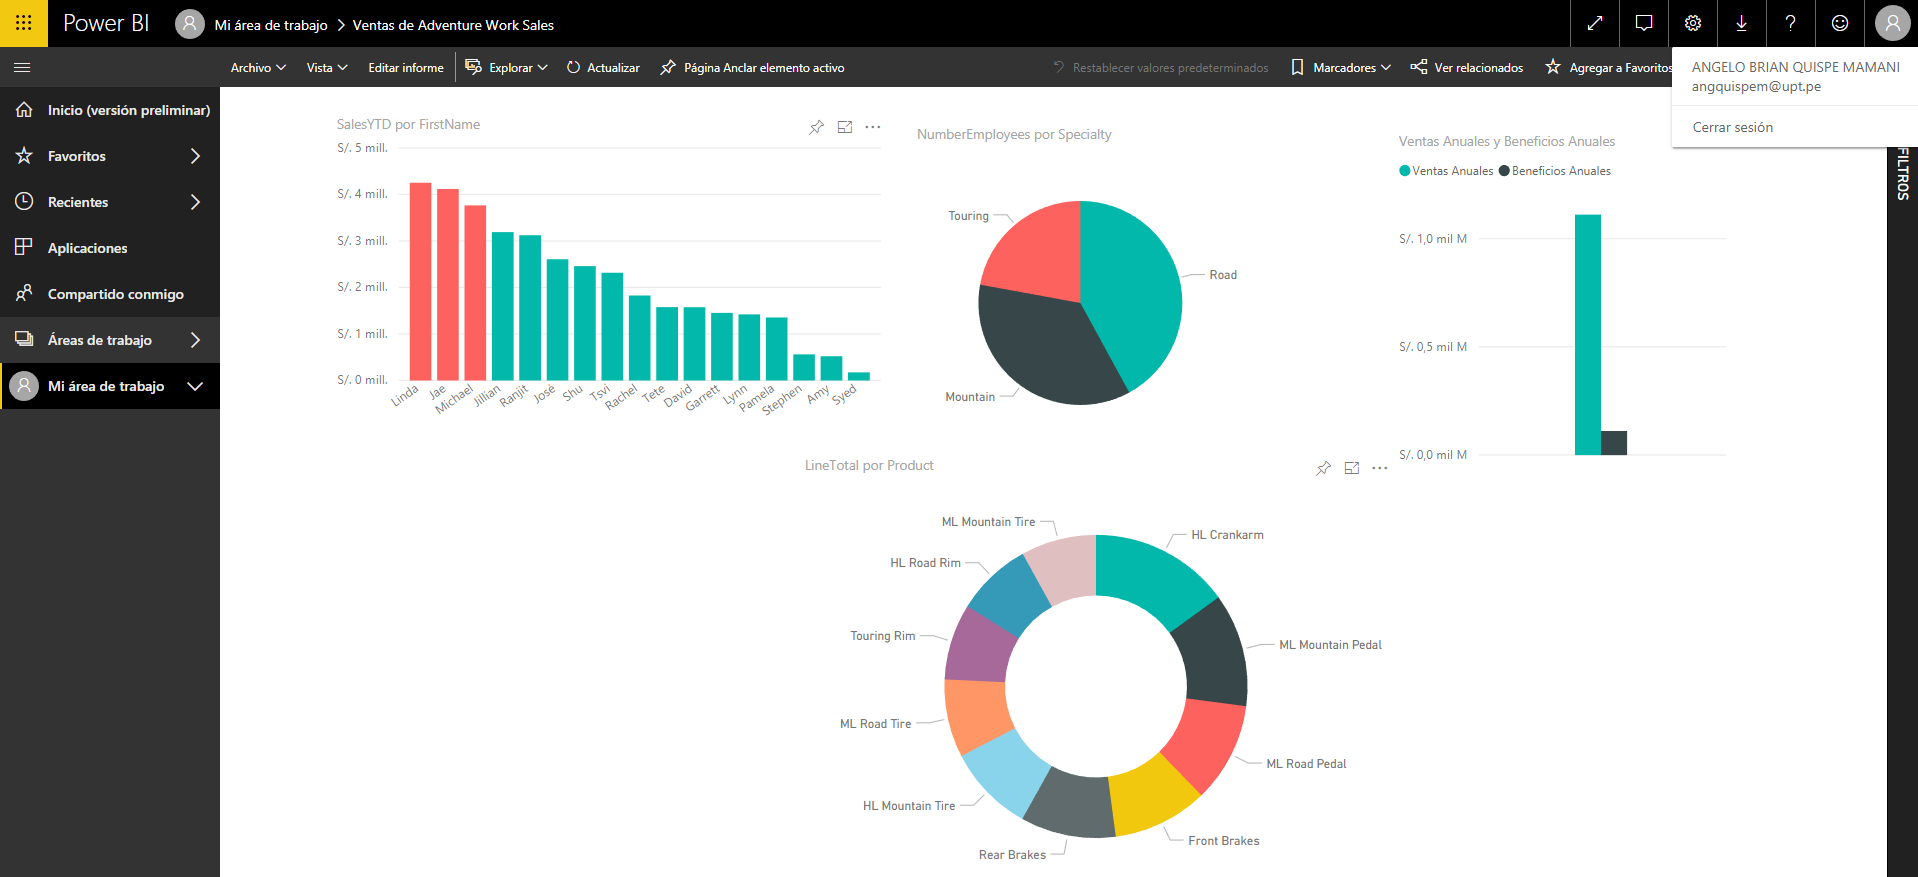
\includegraphics[scale=0.30]{./Imagenes/28.png}
\end{center}



\end{enumerate}









\end{itemize}







